%%%%%%%%%%%%%%%%%%%%%%%%%%%%%%%%%%%%%%%%%%%%%%%%%%%%%%%%%%%%%%%%%%%%%%%%%%%%%%%
\section{OpenMC}
\label{sec:openmc}
%%%%%%%%%%%%%%%%%%%%%%%%%%%%%%%%%%%%%%%%%%%%%%%%%%%%%%%%%%%%%%%%%%%%%%%%%%%%%%%


%%%%%%%%%%%%%%%%%%%%%
\subsection{Overview}
\label{subsec:openmc-overview}


%%%%%%%%%%%%%%%%%%%%%%%
\subsection{Python API}
\label{subsec:pyapi}

A fully-featured Python Application Programming Interface (API) was designed and implemented to enable programmatic pre- and post-processing for OpenMC\cite{boyd2016bigdata}. The API enables tight coupling of input generation, simulation execution, and tally data analysis within dynamic Python script ``input files.'' In addition, the API makes it possible to leverage the extensive ecosystem of Python packages for scientific computing alongside OpenMC in a simulation workflow. The following sections describe the API and some of the core features which comprise the software stack developed to support the MGXS generation module created for OpenMC.

%%%%%%%%%%%%%%%%%%%%%%%%%%%%%%%%%%%%%
\subsubsection{Workflow Organization}
\label{subsubsec:pyapi-workflow}

The Python API is a user-friendly, complementary (and optional) addition to the OpenMC codebase. OpenMC is written in Fortran 2008 and uses eXtensible Markup Language (XML) input files to describe the simulation materials, geometry, tallies, and settings. Although XML is often hailed as both human-readable and machine-readable, it is cumbersome to write by hand for large and complicated reactor models such as those modeled in this thesis. The Python API circumvents this process by leveraging Python's internal \texttt{ElementTree} API to generate the XML files used by the OpenMC executable. Instead of writing XML files by hand, dynamic Python scripts are used to describe one or more OpenMC simulations, including those used to generate MGXS with OpenMC.

The OpenMC Python API adheres to object-oriented software design principles with extensible class definitions. A user instantiates, manipulates, and connects objects representing items such as the materials, geometry and tallies to construct an OpenMC simulation. This is a scalable alternative workflow to traditional ``decks'' of ``cards'' in which data characterizing a simulation is specified in opaque ASCII files (\textit{e.g.}, integer identifiers for geometric primitives such as surfaces, cells, universes, etc.). The Python API provides classes and routines to represent all features provided by OpenMC's XML input specifications.

In addition to its functionality for input generation, the Python API also includes a rich framework of tally data processing utilities. The API eliminates the time intensive and error prone process of writing code to parse results from OpenMC's output files. The API is able to reconstruct the hierarchy of interconnected Python objects used to represent the materials, geometry and tallies from OpenMC's ``statepoint'' and ``summary'' HDF5 output files\cite{koranne2011hdf5}. OpenMC's dynamic object-oriented data processing model -- fusing the geometry and materials configuration with tallied data -- enables the rapid calculation, indexing and storage of MGXS from tallies on unstructured meshes.

%%%%%%%%%%%%%%%%%%%%%%%%%%%%%%%%%
\subsubsection{Pandas DataFrames}
\label{subsubsec:chap4-pandas-df}

The Python API encapsulates numerical tally data using $N$-dimensional array objects from the NumPy package\cite{walt2011numpy}. Although OpenMC's NumPy interface to tally data is more flexible than simply reporting the data in ASCII files, NumPy arrays are relatively opaque containers for managing large tally datasets. A single OpenMC \texttt{Tally} object used for MGXS generation may encompass many different energy groups, nuclides and reaction types, yet all of this data is tabulated in a single contiguous NumPy array. As a result, it is challenging to implement general algorithms to inspect, index, and manipulate tally data in NumPy arrays for specific groups, nuclides or reactions.

The Pandas Python package\cite{mckinney2010pandas} was implemented in the Python API to enable transparent tally data processing for MGXS generation. In particular, the \texttt{Tally} class includes a feature to construct a Pandas \texttt{DataFrame} object from tally data. Pandas DataFrames are modeled after data structures in the \textsf{R} programming language used to store data tables in a more accessible format than contiguous arrays. Pandas DataFrames support mixed-type data (\textit{i.e.}, strings and numbers), and allow the use of string keys or labels to index each column or row. The Python API builds Pandas DataFrames by annotating tally data with the filters, nuclides, and scores associated with each tally bin. 

%%%%%%%%%%%%%%%%%%%%%%%%%%%%%%%%
\subsubsection{Tally Slicing and Merging}
\label{subsubsec:tally-slice-merge}

Two useful and related features in the OpenMC Python API for MGXS generation are \textit{tally merging} and \textit{tally slicing} as depicted in \autoref{fig:tally-merge-slice}. It is intuitively useful to systematically create individual \texttt{Tally} objects for each spatial zone and reaction type when generating the OpenMC inputs necessary to compute MGXS. However, this necessarily leads to a large number (10$^2$ -- 10$^3$) of distinct tally objects for large, complex geometries, which poses a computational bottleneck since the overhead to tally in OpenMC scales as $\mathcal{O}(N)$ for $N$ tallies. To compensate for this, the Python API's \texttt{Tally} class automatically merges user-specified tallies for input generation. Similarly, the API supports the slicing of tallies to simplify downstream data processing which may comprise energy-, nuclide-, and/or reaction-dependent transformations of the tally data.

\begin{figure}
\begin{subfigure}{\textwidth}
  \centering
  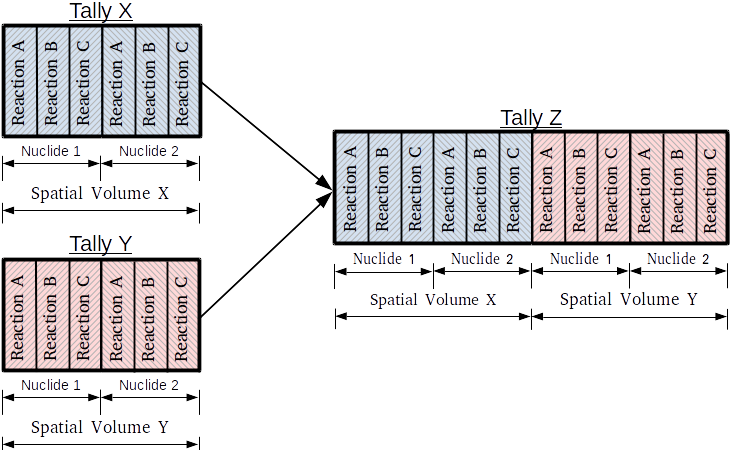
\includegraphics[width=0.8\linewidth]{figures/tally-merge}
  \caption{}
\end{subfigure}
\begin{subfigure}{\textwidth}
  \centering
  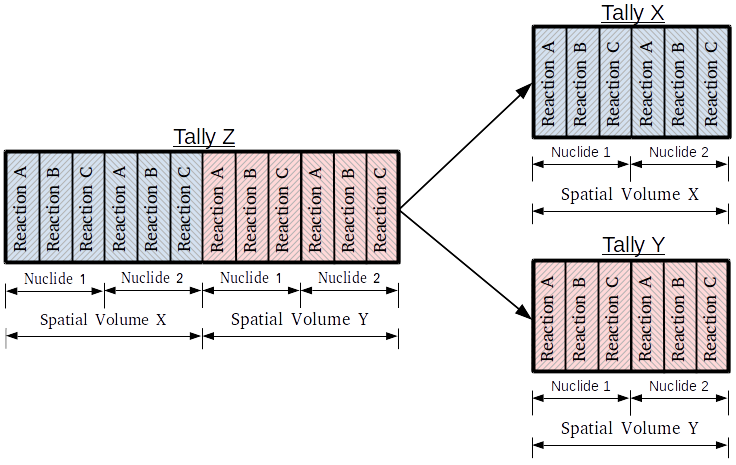
\includegraphics[width=0.8\linewidth]{figures/tally-slice}
  \caption{}
\end{subfigure}
\caption{Two \texttt{Tally} objects for different spatial volumes are merged into a single \texttt{Tally} (a). A single \texttt{Tally} is sliced by spatial volume into two distinct \texttt{Tally} objects (b).}
\label{fig:tally-merge-slice}
\end{figure}

%%%%%%%%%%%%%%%%%%%%%%%%%%%%%%%%
\subsubsection{Tally Arithmetic}
\label{subsubsec:tally-arithmetic}

A variety of reaction rate and flux tallies must be arithmetically combined in order to compute MGXS with Monte Carlo. At the most general level, a reaction rate tally must be divided by a flux tally for each energy group, nuclide and tally volume. The Python API provides a novel feature known as \textit{tally arithmetic} to enable arithmetic combinations of tallies with efficient vectorized numerical operations across energy groups, nuclides and spatial tally zones.

Tally arithmetic is an object-oriented data processing feature which arithmetically combines two or more tallies and/or scalar values into new \textit{derived tallies}. The tally arithmetic implementation in OpenMC overloads the operators for addition, subtraction, multiplication, division, and exponentiation in the Python API's \texttt{Tally} class. In addition, the \texttt{Tally} class supports summation or averaging operations across some or all of its filter, nuclide or score bins. The derived tallies produced from tally arithmetic provide the same rich functionality available for the \texttt{Tally} operands used in the arithmetic operation (\textit{e.g.}, Pandas DataFrames, tally arithmetic).

Multi-group cross sections may be simply and efficiently computed with tally arithmetic. For example, the following code snippet illustrates how tally slicing and arithmetic are used to compute a total MGXS. The total MGXS that is returned from the tally division operation is encapsulated within a \texttt{Tally} class. This is the approach used by the MGXS generation module created for OpenMC.

\lstinputlisting[language=Python, basicstyle=\ttfamily\scriptsize, caption={MGXS calculation with tally arithmetic.}, label={lst:python-input}]{listings/tally-arithmetic.py}

A primary objective of tally arithmetic is to rapidly transform tally data with automated uncertainty propagation. Estimates of the variance for derived tallies from tally arithmetic are deduced from standard error propagation theory~\cite{bevington2003data}. The division arithmetic operator is primarily used to to compute MGXS from MC tallies. Consider two random variables $X$ and $Y$, generated from distributions with variances $\sigma_{X}^2$ and $\sigma_{Y}^2$ which are divided into a new random variable $Z$ with variance $\sigma_{Z}^2$:

\begin{equation}
\label{eqn:div-prop}
\sigma_{Z}^{2} \approx Z^{2}\left[\left(\frac{\sigma_{X}}{X}\right)^{2} + \left(\frac{\sigma_{Y}}{Y}\right)^{2} - 2\frac{\sigma_{XY}}{Z}\right]
\end{equation}

\noindent The random variables $X$ and $Y$ may correspond to tallies for reaction rates and the flux, while $Z$ could correspond to a MGXS.

The covariance $\sigma_{XY}$ of $X$ is not generally computable using the standard formulation for a tally estimator in a Monte Carlo simulation. Although it would be possible to estimate the covariance using ensemble statistics, this is not often feasible. Instead, the covariance term in \autoref{eqn:div-prop} is neglected by the current implementation of tally arithmetic. In general, the random variables for reaction rates and fluxes in the same volume of phase space are highly correlated, such that a conservative estimate of the variance for MGXS is obtained by neglecting the covariance.

%%%%%%%%%%%%%%%%%%%%%%%%%%%%%%%%%%%%%
\subsection{Distributed Cell Tallies}
\label{subsec:distribcells}

Many Monte Carlo codes, including OpenMC, use some variant of combinatorial geometry (CG) because it can represent arbitrary, repeating geometries such as fuel pins and assemblies. However, the CG approach is challenged by applications which require tallies in each instance of a repeated cell throughout a reactor geometry. The ``brute force'' solution is to instantiate a unique cell for each distinct tally zone. However, this defeats the purpose of using CG for its compact representation, and it is not scalable to problems with large tally datasets such as those considered in this thesis.

The \textit{distributed cell tally} algorithm was implemented in OpenMC \cite{lax2014distribcell} to permit simply defined spatial tally zones across repeated cell instances. The distributed cell algorithm, commonly abbreviated as the \textit{distribcell} algorithm, classifies each unique cell instance using an algorithm which consume orders of magnitude less memory than would be required by the ``brute force'' approach. Only a single transparent line of XML input is necessary to define a distribcell tally which may span across an arbitrary number of instances for a particular cell. Furthermore, the Python API may be used to perform efficient vectorized transformations of distribcell tally data stored as contiguous NumPy arrays. In particular, the distribcell tally algorithm may be used to compute spatially-varying MGXS across fuel pin cell instances.

%%%%%%%%%%%%%%%%%%%%%%%%%%%%%
\subsection{Multi-Group Mode}
\label{subsec:openmc-mg-mode}

\begin{itemize}[noitemsep]
\item support stochastic multi-group calculations
\item multiple scattering representations (Legendre moments, discrete bins)
\item use OpenMC to generate MGXS, then insert into identical model for MG calculation
\item mention angular-dependent MGXS, or save for later paper?
\end{itemize}